\DocumentMetadata{tagging=on, pdfstandard=ua-2}

\documentclass[11pt,a4paper]{article}

\usepackage[T1]{fontenc}
\usepackage{graphicx}
\usepackage{tikz}

\graphicspath{{figures/}}

\title{Test document: every .alt state}
\author{u22534599}
\date{}

\InputIfFileExists{_alt/main.alt.tex}{}{}
\begin{document}
\maketitle

\section{Machine-owned states}

\begin{figure}[h]
  \centering
  
\includegraphics[width=0.45\linewidth]{new-chart.png}
  \caption{A chart that has never been described.}
  \label{fig:new-chart}
\end{figure}

\begin{figure}[h]
  \centering
  
\includegraphics[width=0.5\linewidth]{fresh-chart.pdf}
  \caption{A chart already described, unchanged since.}
  \label{fig:fresh-chart}
\end{figure}

\begin{figure}[h]
  \centering
  
\includegraphics[width=0.45\linewidth]{stale-chart.png}
  \caption{A chart that was re-plotted after it was described.}
  \label{fig:stale-chart}
\end{figure}

\section{Human-owned states}

\begin{figure}[h]
  \centering
  
\includegraphics[width=0.35\linewidth]{edited-photo.jpg}
  \caption{A photograph whose description a human corrected.}
  \label{fig:edited-photo}
\end{figure}

\begin{figure}[h]
  \centering
  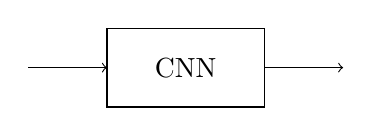
\begin{tikzpicture}
    \draw (0,0) rectangle (2,1) node[midway] {CNN};
    \draw[->] (-1,0.5) -- (0,0.5);
    \draw[->] (2,0.5) -- (3,0.5);
  \end{tikzpicture}
  \caption{A diagram whose description a human signed off.}
  \label{fig:approved-diagram}
\end{figure}

%!alt artifact
\noindent
\includegraphics[width=\linewidth]{divider.png}

\section{Overrides and failures}

\begin{figure}[h]
  \centering
  
\includegraphics[width=0.5\linewidth, alt={Line chart of accuracy against
  training epoch, written by hand in the source.}]{override-chart.pdf}
  \caption{A chart described inline by the author.}
  \label{fig:override-chart}
\end{figure}

\begin{figure}[h]
  \centering
  \includegraphics[width=0.5\linewidth]{absent-chart.pdf}
  \caption{A chart whose file has not been generated yet.}
  \label{fig:absent-chart}
\end{figure}

\begin{figure}[h]
  \centering
  
\includegraphics[width=0.35\linewidth]{unlabelled-photo.jpg}
  \caption{A photograph in a float with no label.}
\end{figure}

\section{Method}

\begin{figure}[h]
  \centering
  
\includegraphics[width=0.45\linewidth]{method-diagram.png}
  \caption{The classification pipeline, drawn as a block diagram.}
  \label{fig:method-diagram}
\end{figure}

This chapter pulls in a section of its own, so the walker has to recurse
rather than only looking one level down.

\subsection{Per-class behaviour}

\begin{figure}[h]
  \centering
  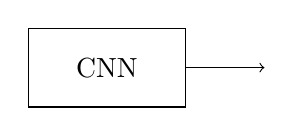
\begin{tikzpicture}
    \draw (0,0) rectangle (2,1) node[midway] {CNN};
    \draw[->] (2,0.5) -- (3,0.5);
  \end{tikzpicture}
  \caption{A classifier block, drawn inline inside a chapter.}
  \label{fig:chapter-tikz}
\end{figure}


\section{Results}

\begin{figure}[h]
  \centering
  
\includegraphics[width=0.5\linewidth]{results-plot.pdf}
  \caption{Test accuracy against training epoch.}
  \label{fig:results-plot}
\end{figure}

\begin{figure}[h]
  \centering
  
\includegraphics[width=0.3\linewidth]{unlabelled-photo.jpg}
  \caption{A photograph keyed by filename, colliding with the one in main.tex.}
\end{figure}


\section{Not figures}

\begin{verbatim}
\begin{figure}
  \includegraphics{in-verbatim.pdf}
  \caption{Shown as text, not included.}
\end{figure}
\end{verbatim}

% \includegraphics[width=2cm]{in-a-comment.png}

\end{document}
